\scanpage{33}
\mspage{32}

% L1–2
1) Pour la relation d'ordre, il y a un plus petit élément $\varnothing$, et un plus grand élément $L$ \inserted{(ou $1$)}.

% L3
2) : $X\subset Y\Rightarrow\{X,Y\}$ modéré

% L4
3) Si $\{X,Y\}$ modéré, $X\wedge Y$ et $X\vee Y$ existent (inf et sup)
% Lleft, opposite 3
% slanted
\margin{- Attention $X\vee Y$ \deleted{\unsure{est|n'}} n'est \uline{pas} l'union \deleted{de} $X\cup Y$ !!}

% L5–6
\deleted{\unsure{3)|3 bis)} Si $\{X,\unsure{Y_i|Y}\}$ \unsure{est|sont} \illegible{2} modérés, alors} \deleted{Si \unsure{deux|les} $X$ \unsure{et|sont} \unsure{modérés} \unsure{pour}} \inserted{(distributivité) et pour une famille d'\unsure{élmt|élémt} mut\textsuperscript{t} mod, $X\wedge(\bigvee_iY_i)=\bigvee_i(X\wedge Y_i)$}

% L7–11
\deleted{\unsure{3|5}}4) \deleted{Parmi les} $\forall X\in\mathcal M$ \deleted{\unsure{éléments|il existe}}, \deleted{\unsure{dans|du}} parmi les $Y\in\mathcal M$ tels que $\{X,Y\}$ modéré, et $X\wedge Y=\varnothing$, il y a un plus grand élément \inserted{$X'$}. C'est aussi l'unique élément tel que
% Lleft, opposite X′ and tel que
% slanted
\margin{\uline{Dire aussi} Si \deleted{\unsure{(élémt)|($X_i$)}} $\{X_i\}_{i\in\unsure{I|J}}\subset\mathcal M$ est formé d'él\textsuperscript{ts} \unsure{mutuellemt|mutuellement} modérés, alors pour les op. $\wedge,\vee,'$ ils engendrent une ``alg. de Boole'', finie si $I$ fini.\figure{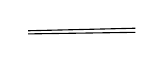
\begin{tikzpicture}[x=.4cm,y=.4cm]\draw (0,0)--(3.4,.08);\draw (0,-.1)--(3.4,-.05);\end{tikzpicture}}}
% L12
\[
\{X',X\}\text{ modéré},\qquad \unsure{X''|X'}\wedge X=\varnothing,\qquad X'\vee X=1
\]
% L13–17
Donc l'application $X\mapsto X'$ est involutive, elle renverse la relation d'ordre (anti-involution), \deleted{donc échange} \deleted{\unsure{De|On}}De plus $\{X\ \mathrm{et}\ Y\}$ sont mod. ssi $\{X',Y'\}$ modéré\textsuperscript{*},
% Lleft of same passage
% slanted
\margin{* En fait, $\forall X,Y$ $\{X,Y\}$ mod. ssi $\{X,Y'\}$ mod (donc ssi $\{X',Y'\}$ mod., \unsure{ssi|et} $\{X',Y\}$ modéré)}
% L18
et alors \quad $(X\wedge Y)'=X'\cup Y'$, \quad $(X\cup Y)'=X'\wedge Y'$

% L19
\deleted{\unsure{4|5}}5) $\varnothing,1\in\mathcal M_f$

% L20–21
\deleted{5}6) $\forall X\in\mathcal M$, il existe un plus petit \deleted{\unsure{4')|$X$|$Y$}} $Y\in\mathcal M_f$ tel que $X\subset Y$ (on pose $Y=\bar X$).
% Lbottom left beside 6
% slanted
\margin{Par passage au compl., on définit $\deleted{\unsure{U|V}}X^{\unsure{\circ|o}}=(\overline{X'})'$.}

% L22–23
De plus Si $X,Y\in\mathcal M$ tels que $\{X,Y\}$ mod, alors $\overline{X\vee Y}=\overline X\vee\overline Y$

% L24 and below
\deleted{6}7) Si $\{X,Y\}$ modéré $\{\overline X,Y\}$ aussi (donc $\{X,\overline Y\}$ et $\{\overline X,\overline Y\}$ aussi
